\thispagestyle{empty}
\vspace{3.0ex}
\begin{center}\uppercase{\normalsize Siglen, Abkürzungen, Zeichen}\end{center}
\vspace{4.0ex}% PR: Rein provisorisch!
\renewcommand*{\chapter}{\OrigChapter}
\noindent\footnotesize
\uppercase{1. Siglen und editorische Zeichen}\\[3.0ex]
\begin{tabular}{lp{110mm}}
\textit{E}, \textit{E}\textsuperscript{1} & Erstdruck\\
\textit{E}\textsuperscript{2} ... & weitere Drucke\\
\textit{L}, \textit{L\textsuperscript{1}} ... & Leibniz, eigenh\"{a}ndig\\
\textit{l} & Leibniz, Abschrift von Schreiberhand\\
\textit{Lil} & Leibniz' eigenh\"{a}ndige Bemerkungen und Verbesserungen in einer Abschrift von Schreiberhand\\
% \textit{A} & fremdhändige Abschrift eines fremden Textes\\
% \textit{LiA} & Leibniz' eigenh\"{a}ndige Bemerkungen und Verbesserungen in einer fremdhändigen Abschrift eines fremden Textes\\
\textit{LiH} & Leibniz' eigenh\"{a}ndige Anstreichungen und Anmerkungen in einem Handexemplar\\
$[~]$ & bei Datierungen: erschlossenes Datum
\newline im Text und bei Abbildungen: Änderungen und Erg\"{a}nzungen des Herausgebers
\newline von Leibniz benutzte eckige Klammern werden im Erl\"{a}uterungs\-apparat angezeigt\\
% \textit{[~]} & vom Herausgeber hinzugef\"{u}gte Figurenbezeichnungen\\
% \textit{(~)} & von Leibniz in Figuren seines Handexemplars hinzugef\"{u}gte Bezeichnungen\\
$\langle$\ $\rangle$ & Konjektur schwer lesbarer oder durch Besch\"{a}digung des Textzeugen ausgefallener W\"{o}rter bzw. Wortteile\\
$\langle$\textendash $\rangle$~$\langle$\textendash~\textendash$\rangle$ & nicht entziffertes bzw. durch Besch\"{a}digung des Textzeugen aus\-gefallenes Wort;
die Anzahl der Striche entspricht der Anzahl der vermuteten W\"{o}rter.\\
\textit{Kursivierung} & Zitierter Titel von Büchern oder Schriften
\newline w\"{o}rtliches oder fast w\"{o}rtliches Zitat;
als \glqq fast w\"{o}rtlich\grqq\ gilt eine Text\-wiedergabe, die unbedeutsam von der Vorlage abweicht,
etwa bei fl\"{u}chtiger Wortfolge oder Kasus\-\"{a}nderungen\\
% ??Text in anderer als der Grundsprache des betreffenden Textes
% \newline ??Herausgebertext\\
\textso{Sperrung} & Hervorhebungen durch Leibniz %Die Art der Hervorhebung wird im Er\-l\"{a}uterungsapparat angezeigt.
\end{tabular}
\vspace*{4.0ex}
%%%%
%%%%

\noindent\footnotesize
\uppercase{2. Abk\"{u}rzungen} (allgemein)
\setlength\LTleft{0pt} \setlength\LTright{0pt}
\begin{longtable}{ll}
a.a.O. & am angegebenen Ort\\
Anm. & Anmerkung\\
Aufl. & Auflage\\
Bd(e) & Band (B\"{a}nde)\\
bes. & besonders\\
Bl. & Blatt\\
Bog. & Bogen\\
bzw.  & beziehungsweise\\
c. & caput (capita), capitulum (capitula)\\
ca. & circa\\
cap. & caput (capita), capitulum (capitula)\\
ebd. & ebenda\\
e.g. & exempli gratia\\
erg. & erg\"{a}nzt\\
Erl. & Erläuterung\\
Fig. & Figur\\
f. (ff.)& folgend(e)\\
% ff. & folgende\\
gestr. & gestrichen\\
GWLB & Gottfried Wilhelm Leibniz Bibliothek \textendash\ Niedersächsische Landesbibliothek\\
Hrsg. (hrsg.) & Herausgeber (herausgegeben)\\
Jh. & Jahrhundert\\
% k.E. & kein Eintrag\\
l. & liber (libri)\\
LBr & \textsc{Hannover}, GWLB, Leibniz-Briefwechsel\\
LH & \textsc{Hannover}, GWLB, Leibniz-Handschriften\\
lib. & liber (libri)\\
m. & mit\\
Marg. & Marginalie(n)\\
Ms. & Manuskript\\
n. & numerus (numeri)\\
N. & Stücknummer(n) in der \textit{LSB}-Ausgabe\\
NB & nota bene\\
Nr. & Nummer(n)\\
Nachdr. & Nachdruck\\
o.S. & ohne Seitenangabe\\
p. & pagina(e), page(s)\\
r\textsuperscript{o} & recto\\
% RS & Royal Society\\
S. & Seite(n)\\
s.a. & siehe auch\\
s.o. & siehe oben\\
Sp. & Spalte(n)\\
s.u. & siehe unten\\
SV & Schriftenverzeichnis\\
% TD & Teildruck\\
tlw. & teilweise\\
u.a. & und andere, unter anderem\\
v. & van, von\\
Var. & Variante\\
v.c. & verbi causa\\
v.g. & verbi gratia\\
vgl. & vergleiche\\
% vermutl. & vermutlich\\
v\textsuperscript{o} & verso\\
Z. & Zeile(n)\\
z.B. & zum Beispiel
\end{longtable}
\vspace{2.0ex}
%\clearpage
\noindent\footnotesize{\uppercase{3. Abk\"{u}rzungen} (Schriften)}\par
\vspace{2.0ex}
%%%%
%%%%

%\setlength\LTleft{0pt} \setlength\LTright{0pt}
%\begin{longtable}{lp{105mm}}
\noindent\hangindent=10mm\textit{BH:} T. \textsc{Birch}, \textit{The History of the Royal Society of London for improving of natural knowledge: from its first rise}, London 1757.\par
%
\noindent\hangindent=10mm\textit{BW:} R. \textsc{Boyle}, \textit{The Works}, hrsg. von M. Hunter und E. B. Davis, London 1999ff.\par
%
\noindent\hangindent=10mm Cc 2: \textit{Catalogue critique des manuscrits de Leibniz, Fascicule  II (Mars 1672\textendash Novembre 1676)}, hrsg. von A. Rivaud u.a., Poitiers 1914\textendash 1924.\par
%
\noindent\hangindent=10mm\textit{DO:} R. \textsc{Descartes}, \textit{Oeuvres}, hrsg. von C. Adam u. P. Tannery, 12 Bde, Paris 1879\textendash 1910, 2. Aufl. ebd. 1964\textendash 1972.\par
%
% \noindent\hangindent=10mm\textsc{Dutens}: \textsc{Leibniz, G. W.}, \textit{Opera omnia, nunc primum collecta, in classes distributa, praefationibus et indicibus exornata}, hrsg. von L. Dutens, 6 Bde, Genf 1768; Nachdr. Hildesheim 1989.\par
%
\noindent\hangindent=10mm\textsc{Gerland} 1906: G.W. \textsc{Leibniz}, \textit{Nachgelassene Schriften physikalischen, mechanischen und technischen Inhalts}, hrsg. von E. Gerland, Leipzig 1906; Nachdr. Hildesheim, New York 1995.\par
%
\noindent\hangindent=10mm\textit{GO:} G. \textsc{Galilei}, \textit{Opere. Edizione Nazionale}, hrsg. von A. Favaro u.a., 20 Bde, Florenz 1890\textendash 1909. Neuausgabe von S. Garbasso u.a., Florenz 1929\textendash 1932.\par
%
\noindent\hangindent=10mm\textit{GOO:} P. \textsc{Gassendi}, \textit{Opera omnia}, 6 Bde, Lyon 1658; Nachdr. Stuttgart-Bad Cannstatt 1964.\par
%
\noindent\hangindent=10mm\textit{HO:} C. \textsc{Huygens}, \textit{Oeuvres compl\`{e}tes}, hrsg. von D. Bierens de Haan, J. Bosscha u.a., 22 Bde, Den Haag 1888\textendash 1950.\par
%
\noindent\hangindent=10mm\textit{JS:} \textit{Journal des S\c{c}avans}, Paris 1665ff.\par
%
\noindent\hangindent=10mm\textit{KGW:} J. \textsc{Kepler}, \textit{Gesammelte Werke}, hrsg. von der Bayerischen Akademie der Wissenschaften, M\"{u}nchen 1923ff.\par
%
\noindent\hangindent=10mm KK 1: \textit{Kritischer Katalog der Leibniz-Handschriften, 1. Heft 1646\textendash 1672}, hrsg. von P. Ritter, als Manuskript ver\"{o}ffentlicht Berlin 1908.\par
%
\noindent\hangindent=10mm\textit{LSB:} G.W. \textsc{Leibniz}, \textit{S\"{a}mtliche Schriften und Briefe}, Akademie Ausgabe, Darmstadt 1923ff. (seit 1954: Berlin).\par
%
% \noindent\hangindent=10mm\textit{PO:} \textsc{Pascal, B.},	\textit{Oeuvres}, hrsg. von P. Boutroux, L. Brunschvicg, F. Gazier, 14~Bde, Paris 1904\textendash 1914; Nachdr. Vaduz 1965.\par
%
\noindent\hangindent=10mm\textit{PT:} \textit{Philosophical Transactions}, London 1665ff.\par
%
% \noindent\hangindent=10mm\textit{SPW}: \textsc{Stevin, S.}, \textit{The principal works}, hrsg. von E. J. Dijksterhuis u.a., Amsterdam 1955\textendash 1966.\par
%
\noindent\hangindent=10mm\textit{TBO:} T. \textsc{Brahe}, \textit{%Tychonis Brahe Dani 
Opera omnia}, 15 Bde, hrsg. von J.L.E. Dreyer, Kopenhagen 1913\textendash 1929.\par
%
% \noindent\hangindent=10mm\textit{TO:} \textsc{Torricelli, E.}, \textit{Opere}, hrsg. von G. Loria, G. Vassura, 4 Bde, Faenza 1919\textendash 1944.\par
%
\noindent\hangindent=10mm\textit{WO:} J. \textsc{Wallis}, \textit{Opera mathematica}, 3 Bde, Oxford 1693\textendash 1699; Nachdr. Hildesheim 1972.\par
%
%\end{longtable}
\vspace{6.0ex}
%%%%
%%%%

\noindent\footnotesize{\uppercase{4. Alchemische Zeichen}}
\setlength\LTleft{0pt} \setlength\LTright{0pt}
\begin{longtable}{lp{100mm}}
\footnotesize
\earth & Antimon\\
\saturn & Blei (Saturn)\\
\Cancer\ & Krebs\\
\mars & Eisen (Mars)\\
\astrosun & Gold (Sonne)\\
\venus & Kupfer (Venus)\\
\protect
\includegraphics[width=0.02\textwidth]{images/sym-oleum2.pdf} & \"{O}l\\
$\mercury$ & Quecksilber (Merkur)\\
\protect
\includegraphics[width=0.02\textwidth]{images/salpeter2.pdf} & Salpetersäure (Aqua fortis)\\
\protect
\includegraphics[width=0.02\textwidth]{images/sym-sal.pdf} & Salz\\
\protect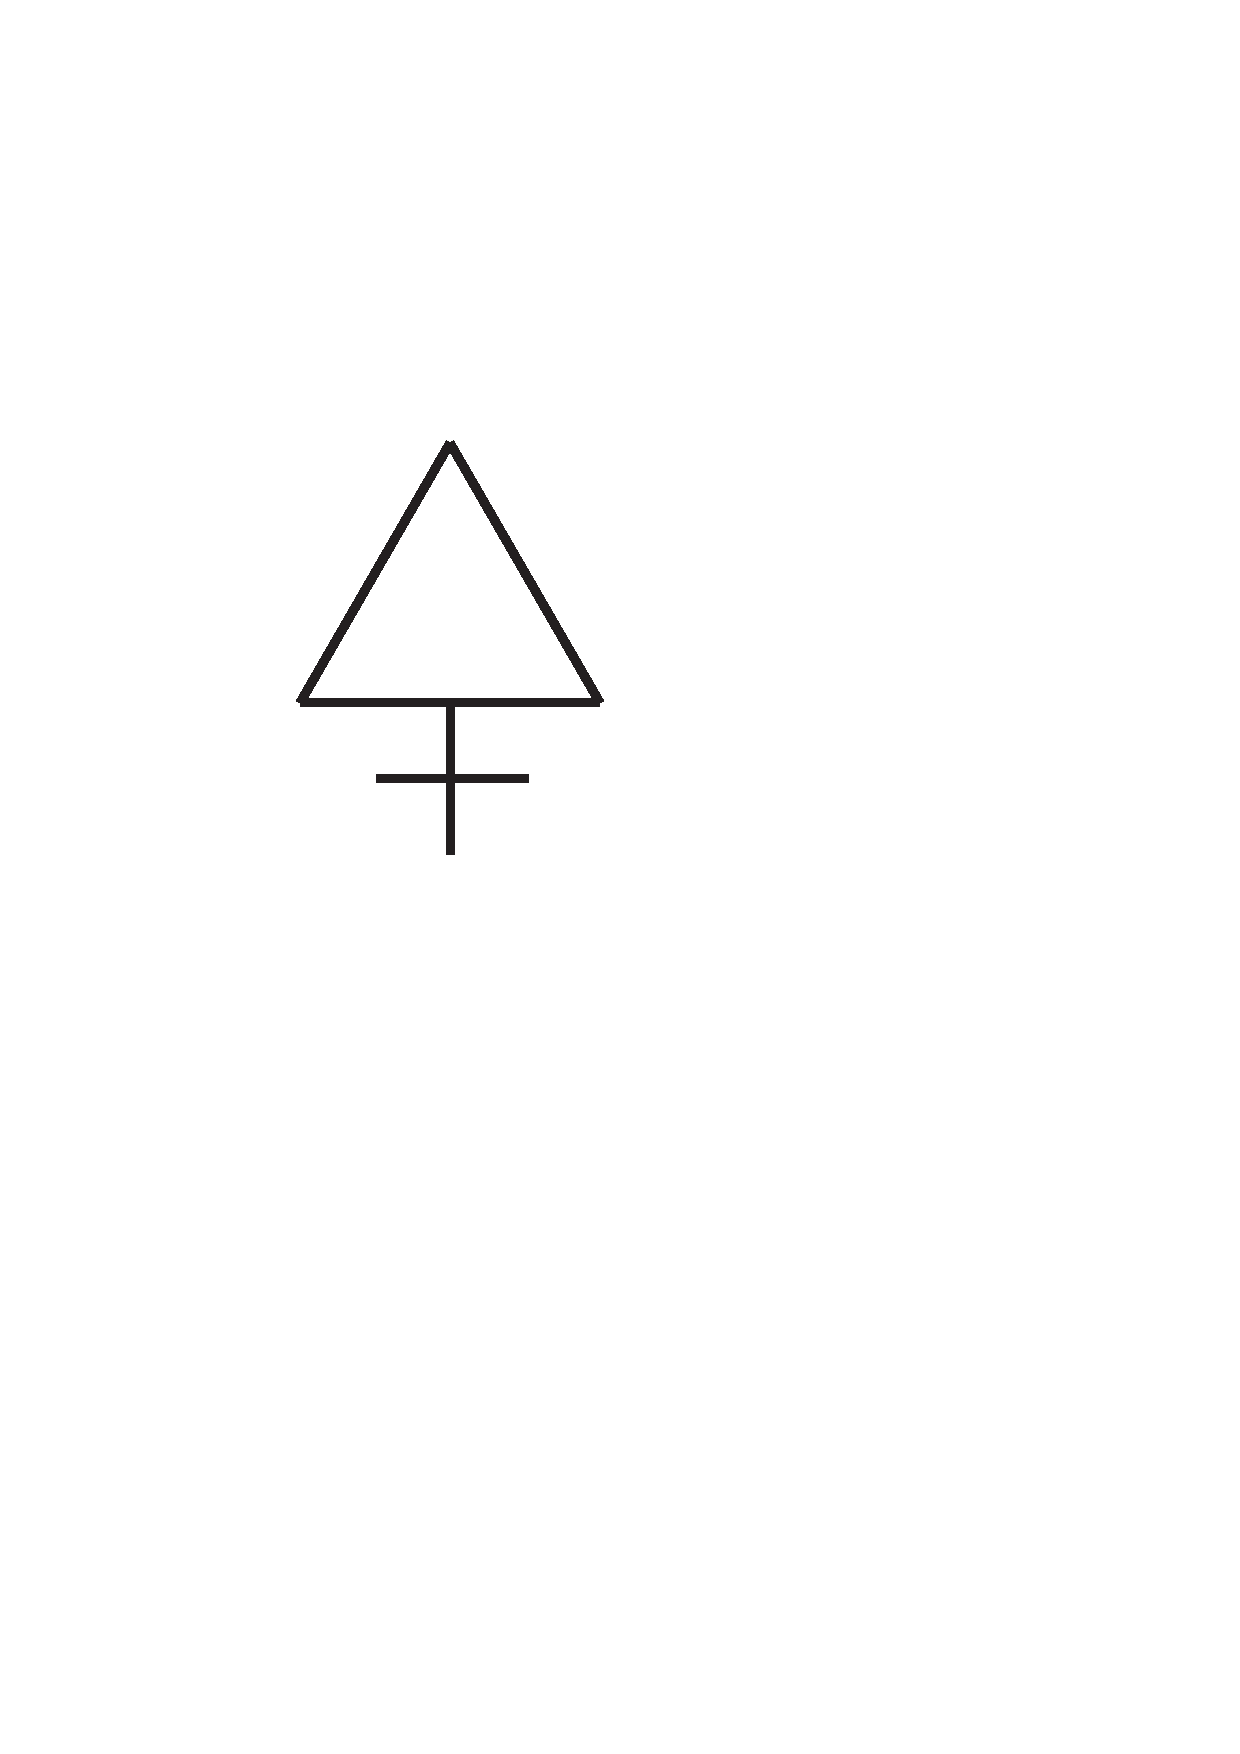
\includegraphics[width=0.02\textwidth]{images/sym-sulph.pdf} & Schwefel\\
$\rightmoon$ & Silber (Mond)\\
% \protect
\includegraphics[width=0.02\textwidth]{images/taros.pdf} & Tartar\\
\protect
\includegraphics[width=0.02\textwidth]{images/vitriol.pdf} & Vitriol\\
$\bigtriangleup$ & Wasser\\
\protect
\includegraphics[width=0.02\textwidth]{images/sym-spirvini.pdf} & Weingeist (Spiritus vini)\\
\protect
\includegraphics[width=0.02\textwidth]{images/taros.pdf} & Weinstein (Tartar)\\
\jupiter & Zinn (Jupiter)
\end{longtable}
\vspace{2.0ex}
%%%%
%%%%
\newpage

\noindent\footnotesize{\uppercase{5. Mathematische Zeichen}}
\setlength\LTleft{0pt} \setlength\LTright{0pt}
\begin{longtable}{lp{100mm}}
\footnotesize\vspace*{1mm}
$\smallfrown$ & Multiplikation\\\vspace*{1mm}
$\smallsmile$ & Division\\\vspace*{1mm}
$\bigtriangledown$ & Dreieck\\\vspace*{1mm}
\rule{1pt}{3mm} & K\"{u}rzung eines Bruchs\\\vspace*{1mm}
$f$ & facit\\\vspace*{1mm}
$\square$ \fbox{2} & Quadrat\\\vspace*{1mm}
\fbox{3}~~cub. & Kubus\\\vspace*{1mm}
$\surd~~~\sqrt{~~~}$\ \ Rq. & Quadratwurzel\\\vspace*{1mm}
=\ aequ.\ aeq.\ $\sqcap$ $\rightpropto$ & gleich\\
$\groesser$ & gr\"{o}{\ss}er als\\
$\kleiner$ & kleiner als\\ \vspace*{1mm}
$\infty$ & unendlich\\
, ,, ,,, $\llcorner \lrcorner$ & Klammerausdr\"{u}cke\\\vspace*{1mm}
\ovalbox{\makebox[15mm][l]{~~~}} & Umrahmungen zur Bezeichnung wegfallender Terme\\\vspace*{1mm}
... & Platzhalter f\"{u}r Terme\\
$\pPsMs$\ $\pleibdashv$ & kombinierte Vorzeichen% $+-$
\\
$\pMsPs$\ $\pleibvdash$% & kombinierte Vorzeichen $-+$
\\
$\pPsPsMs$\ $\ppmE$\ $\ppmG$% & kombinierte Vorzeichen $+(+-)$
\\
$\pPsMsPs$\ $\ppmH$% & kombinierte Vorzeichen $+(-+)$
\\
$\pMsPsMs$%\ & kombinierte Vorzeichen ??$-(+-)$ % oder: plus minus plus ??
\\
$\pMsMsPs$%\ & kombinierte Vorzeichen ??$-(-+)$ % oder: minus plus plus ??
\\
$\pMsPsPs$\ $\ppmD$% & kombinierte Vorzeichen $-(++)$
\end{longtable}
\vspace{2.0ex}
%%%%
%%%%

\noindent\footnotesize{\uppercase{6. Zeichen von Masseinheiten}}
\setlength\LTleft{0pt} \setlength\LTright{0pt}
\begin{longtable}{lp{100mm}}
\footnotesize\vspace*{1mm}
\protect
\includegraphics[width=0.011\textwidth]{images/drachma.pdf} & Drachme\\
\protect
\includegraphics[width=0.022\textwidth]{images/semidrachma.pdf} & halbe Drachme\\\vspace*{1mm}
\protect
\includegraphics[width=0.023\textwidth]{images/semiuncia.pdf} & halbe Unze\\
\Pfund & Pfund\\\vspace*{1,2mm}
\protect
\includegraphics[width=0.018\textwidth]{images/sym-scrupulus.pdf} & Skrupel\\
\protect
\includegraphics[width=0.011\textwidth]{images/uncia.pdf} & Unze
\end{longtable}
\vspace{2.0ex}
%%%%
%%%%

\noindent\footnotesize{\uppercase{7. Sonstige Zeichen}}
\setlength\LTleft{0pt} \setlength\LTright{0pt}
\begin{longtable}{lp{100mm}}
\footnotesize
\Denarius & destilletur, distilletur (noch zu bedenken)\\
\textrecipe & recipe (Rezeptur)
\end{longtable}
\vspace{2.0ex}
%%%%
%%%%


 \newpage
% \vspace*{4.0ex}% PR: Rein provisorisch!
% \renewcommand*{\chapter}{\OrigChapter}


% \noindent\normalsize{\uppercase{Sonderzeichen für Herrn Bayuk}}\vspace*{3mm}
% \setlength\LTleft{0pt} \setlength\LTright{0pt}
% \begin{longtable}{lp{100mm}}
% \normalsize\vspace*{3mm}
% $\pmA$\ $\ppmA$ & \textit{Bedeutung:} $-(-+)$ \ \textit{Befehl:} $\backslash$pmA \textit{bzw.} $\backslash$ppmA \textit{(gesenkt)}\\
% $\pmB$\ $\ppmB$ & \textit{Bedeutung:} $-(+-)$ \ \textit{Befehl:} $\backslash$pmB \textit{bzw.} $\backslash$ppmB \textit{(gesenkt)}
% \end{longtable}
% \vspace{2.0ex}
%%%%
%%%%
